\chapter{Results} \label{cp:results}

\section{Pressure Distribution}
\autoref{fig:measured_vs_theoretical_pressure} compares the theoretical and measured pressure distribution along the nozzle at four different conditions: the 1st, 2nd, and 3rd Critical Conditions along with when there is a normal shock in the nozzle. 

\begin{figure}
    \centering
    \begin{subfigure}{0.49\textwidth}
        \centering
        \includesvg[width=\textwidth]{Figures/Measured vs. Theoretical Pressure Distribution - 1st Critical Condition.svg}
        \caption{Flow is at the first critical condition.}
        \label{fig:measured_vs_theoretical_pressure_1st_critical}
    \end{subfigure}
    \begin{subfigure}{0.49\textwidth}
        \centering
        \includesvg[width=\textwidth]{Figures/Measured vs. Theoretical Pressure Distribution - Normal Shock Inside the Nozzle.svg}
        \caption{Flow has a normal shock.}
        \label{fig:measured_vs_theoretical_pressure_normal_shock}
    \end{subfigure} \\
    \begin{subfigure}{0.49\textwidth}
        \centering
        \includesvg[width=\textwidth]{Figures/Measured vs. Theoretical Pressure Distribution - 2nd Critical Condition.svg}
        \caption{Flow is at the second critical condition.}
        \label{fig:measured_vs_theoretical_pressure_2nd_critical}
    \end{subfigure}
    \begin{subfigure}{0.49\textwidth}
        \centering
        \includesvg[width=\textwidth]{Figures/Measured vs. Theoretical Pressure Distribution - 3rd Critical Condition.svg}
        \caption{Flow is at the third critical condition.}
        \label{fig:measured_vs_theoretical_pressure_3rd_critical}
    \end{subfigure}
    \caption{Plots of the measured and theoretical pressure distribution in the de Laval nozzle.}
    \label{fig:measured_vs_theoretical_pressure}
\end{figure}

\newpage

\section{Mach Distribution}

\begin{figure}[htpb]
    \centering
    \begin{subfigure}{0.49\textwidth}
        \centering
        \includesvg[width=\textwidth]{Figures/Measured vs. Theoretical Mach Number - 1st Critical Condition.svg}
        \caption{Flow is at the first critical condition.}
        \label{fig:measured_vs_theoretical_mach_1st_critical}
    \end{subfigure}
    \begin{subfigure}{0.49\textwidth}
        \centering
        \includesvg[width=\textwidth]{Figures/Measured vs. Theoretical Mach Number - Normal Shock Inside the Nozzle.svg}
        \caption{Flow has a normal shock.}
        \label{fig:measured_vs_theoretical_mach_normal_shock}
    \end{subfigure} \\
    \begin{subfigure}{0.49\textwidth}
        \centering
        \includesvg[width=\textwidth]{Figures/Measured vs. Theoretical Mach Number - 2nd Critical Condition.svg}
        \caption{Flow is at the second critical condition.}
        \label{fig:measured_vs_theoretical_mach_2nd_critical}
    \end{subfigure}
    \begin{subfigure}{0.49\textwidth}
        \centering
        \includesvg[width=\textwidth]{Figures/Measured vs. Theoretical Mach Number - 3rd Critical Condition.svg}
        \caption{Flow is at the third critical condition.}
        \label{fig:measured_vs_theoretical_mach_3rd_critical}
    \end{subfigure}
    \caption{Plots of the measured and theoretical Mach distribution in the de Laval nozzle.}
    \label{fig:measured_vs_theoretical_mach}
\end{figure}

\newpage

\section{Schlieren Images}

\begin{figure}[htpb]
    \centering
    \begin{subfigure}{0.49\textwidth}
        \centering
        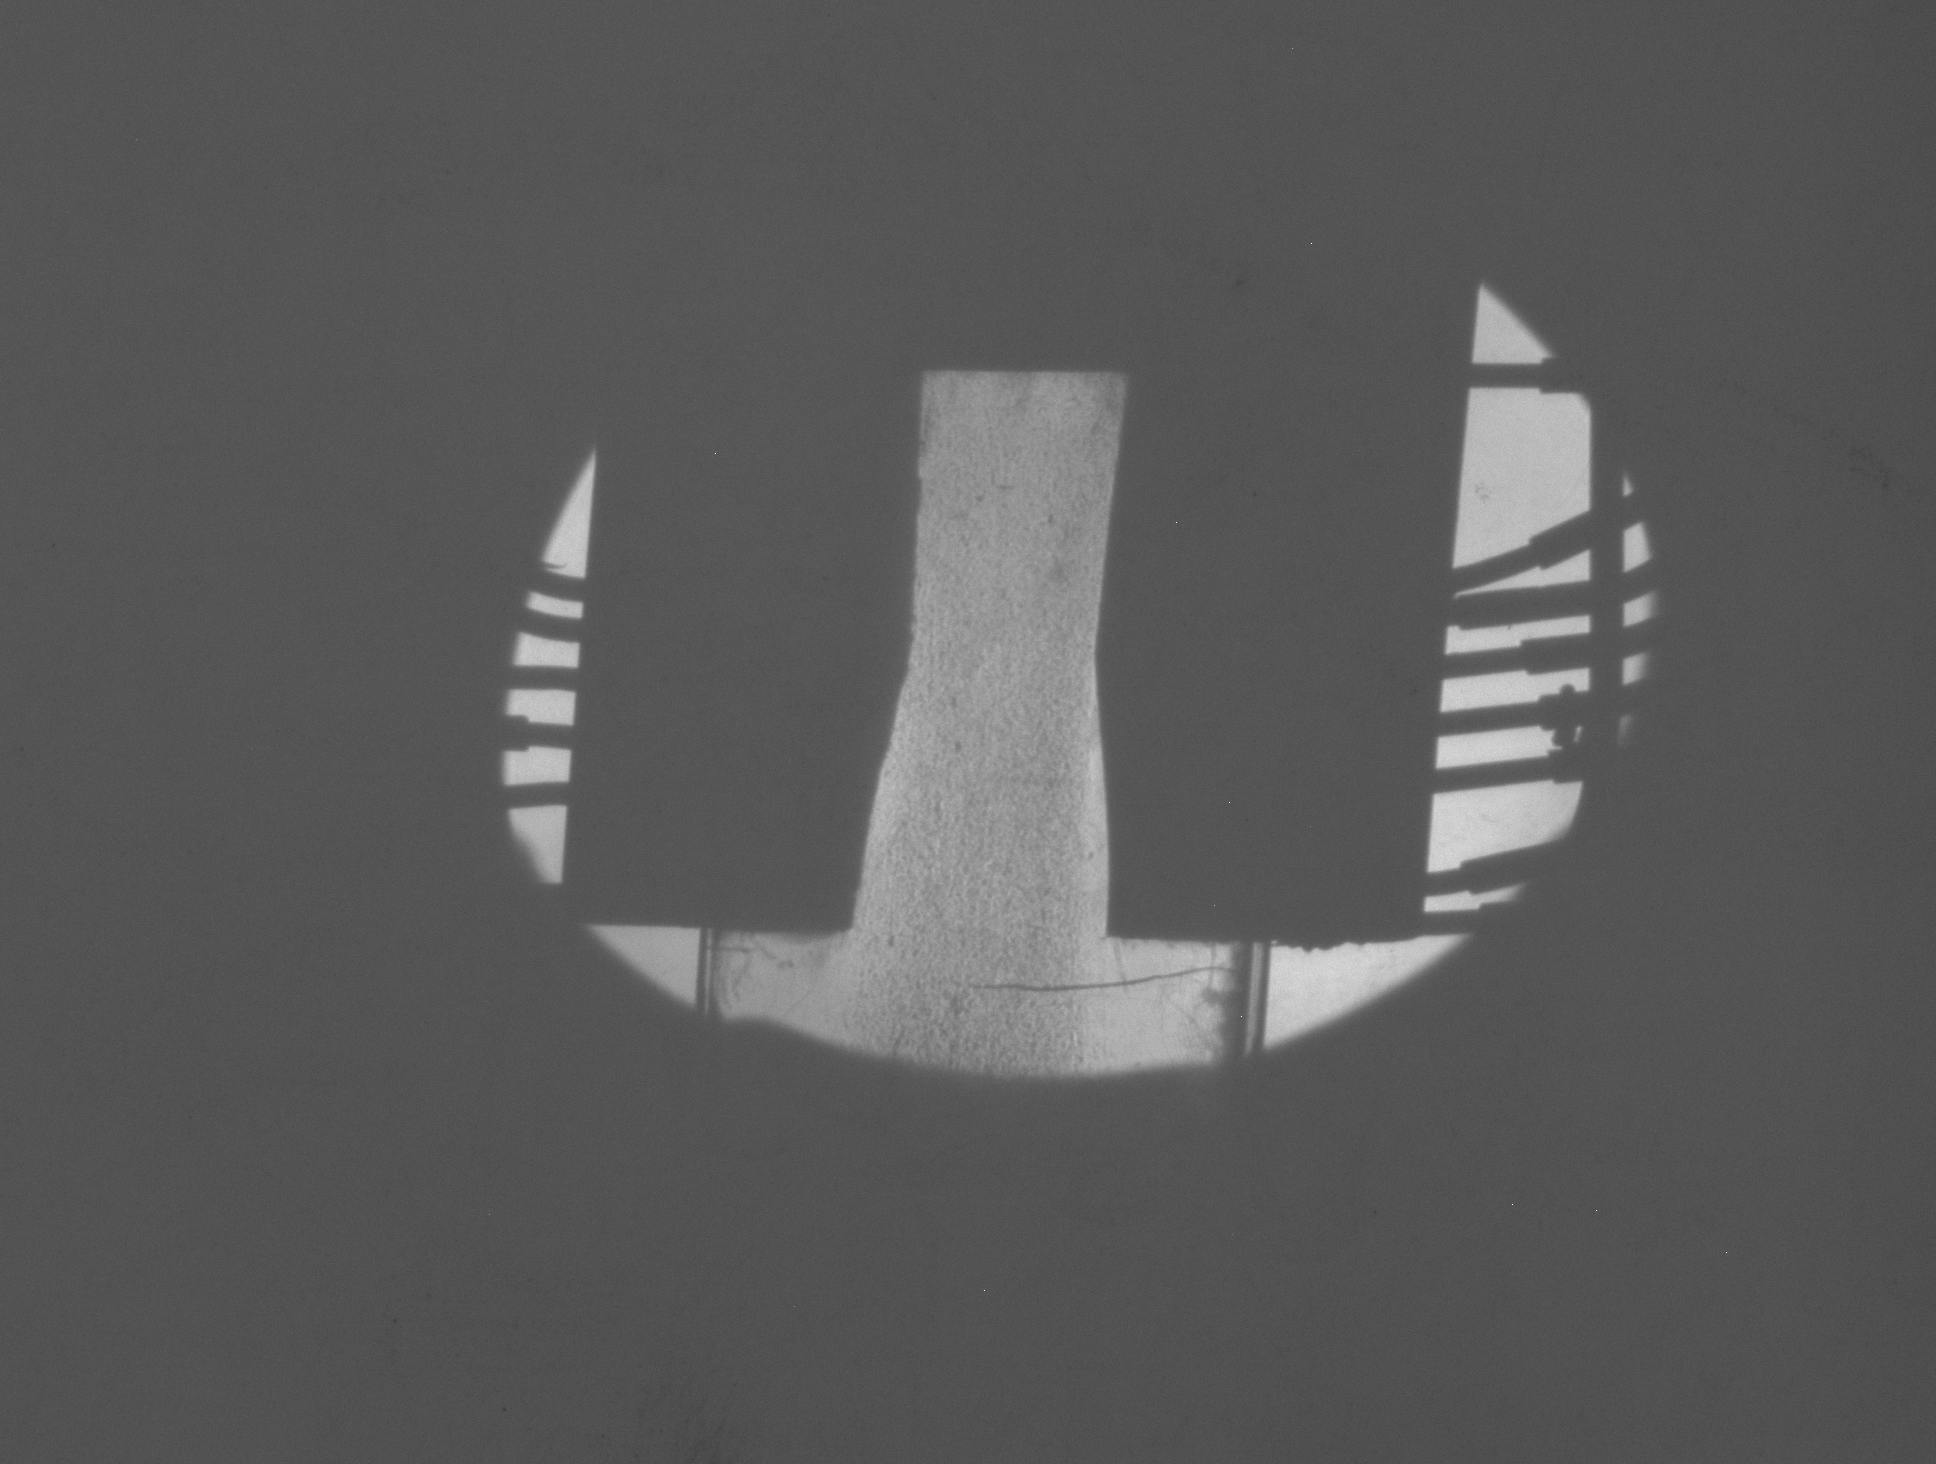
\includegraphics[width=\textwidth]{Figures/6-1st_critical_condition.tiff}
        \caption{Flow is at the first critical condition.}
        \label{fig:schlieren_first_critical}
    \end{subfigure}
    \begin{subfigure}{0.49\textwidth}
        \centering
        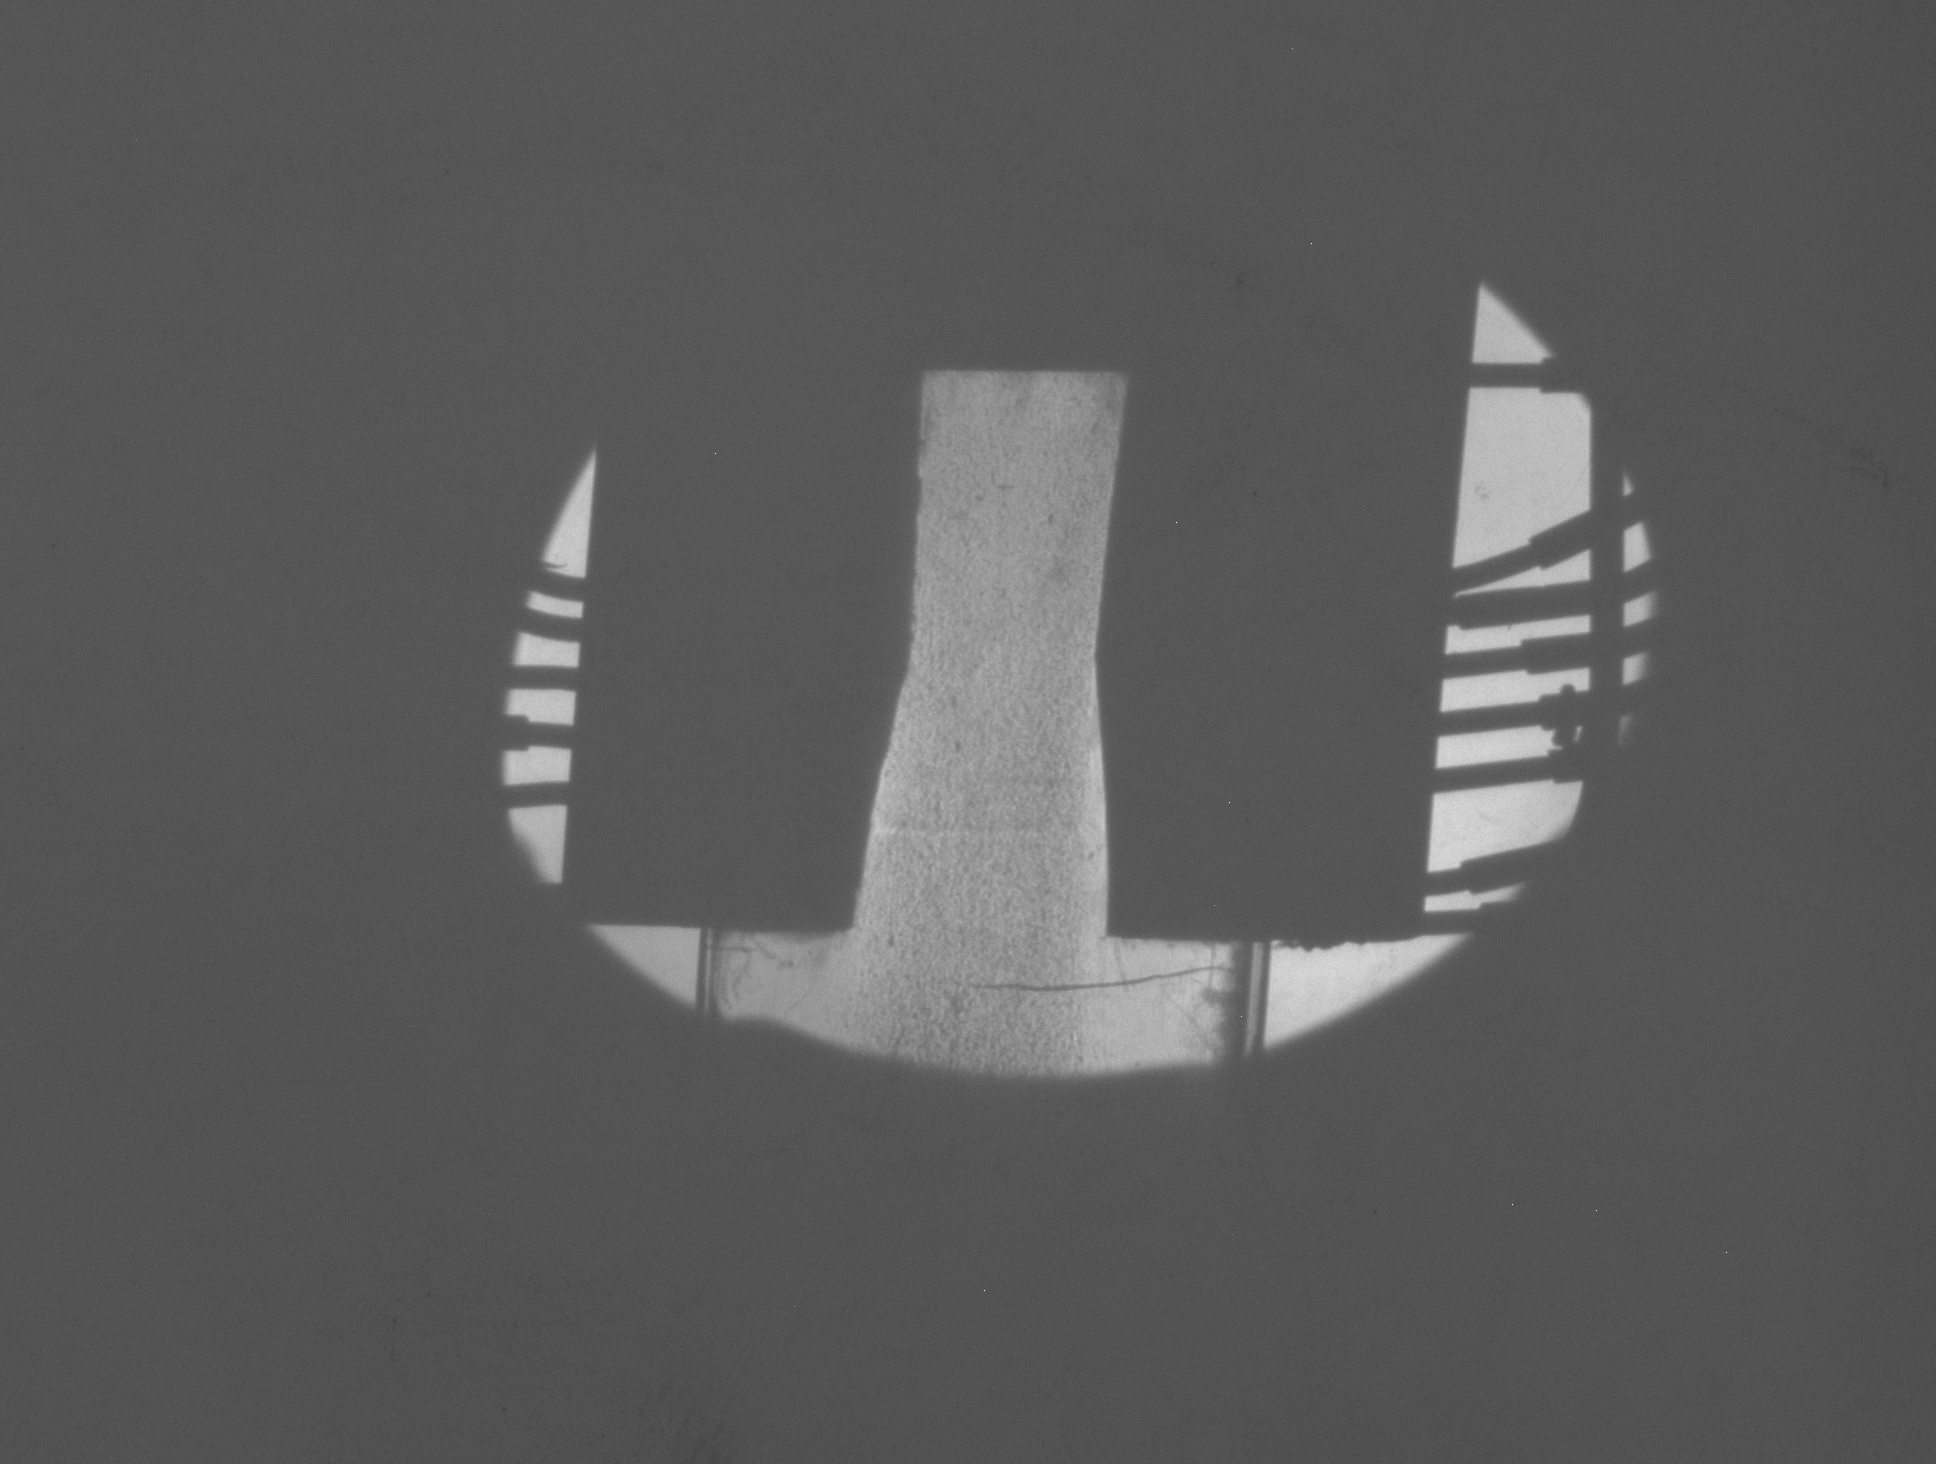
\includegraphics[width=\textwidth]{Figures/5-normal_shock_inside.tiff}
        \caption{Flow has a normal shock.}
        \label{fig:schlieren_normal_shock}
    \end{subfigure} \\
    \begin{subfigure}{0.49\textwidth}
        \centering
        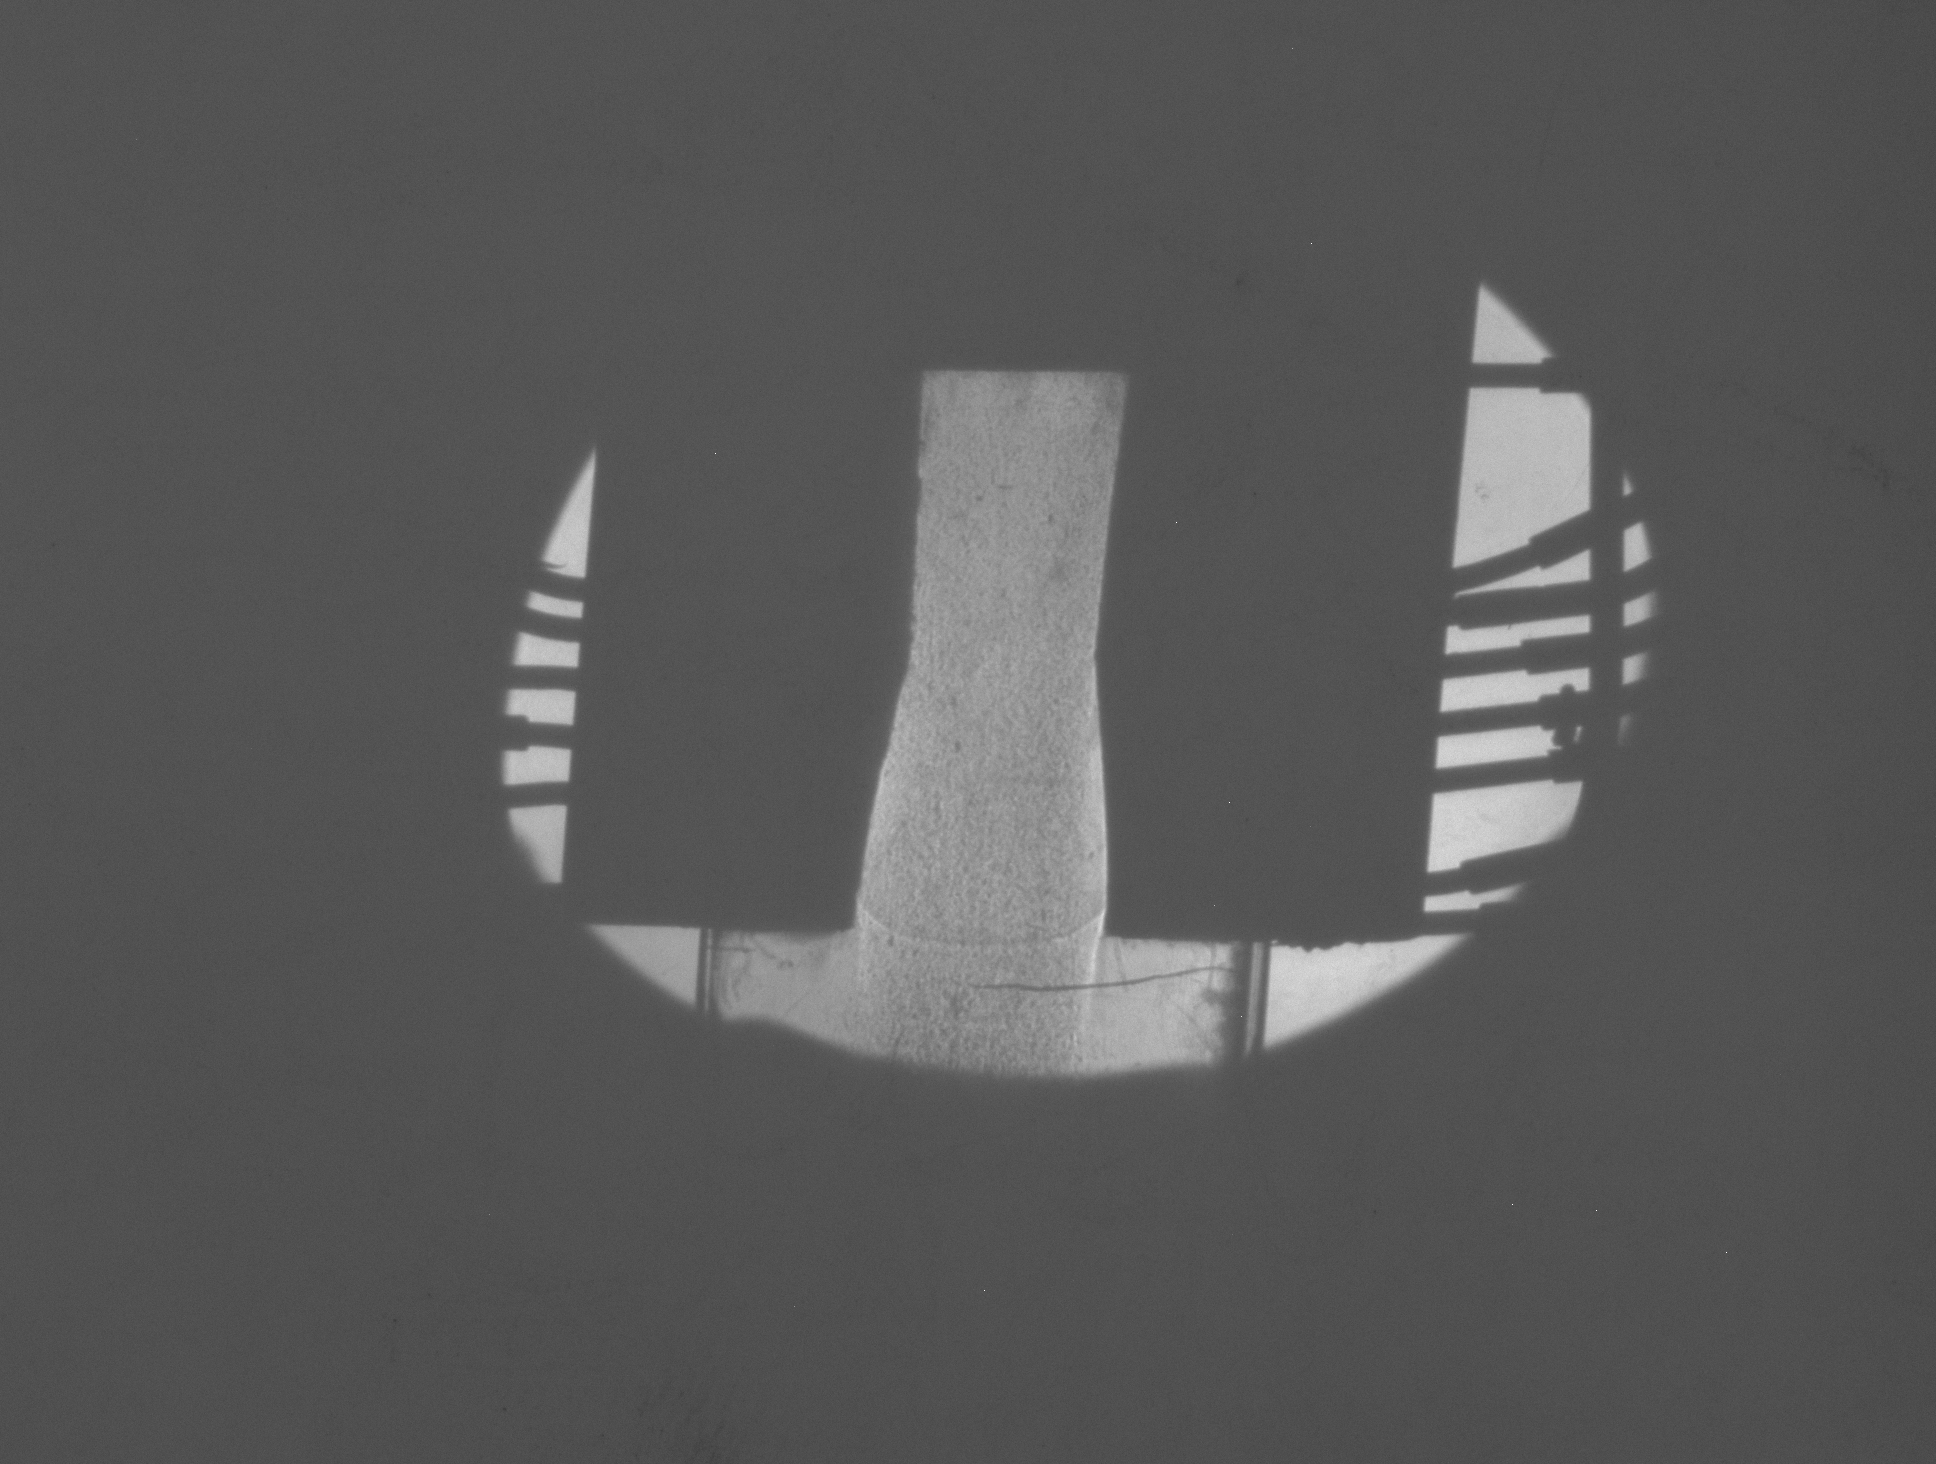
\includegraphics[width=\textwidth]{Figures/4-2nd_critical_condition.tiff}
        \caption{Flow is at the second critical condition.}
        \label{fig:schlieren_second_critical}
    \end{subfigure}
    \begin{subfigure}{0.49\textwidth}
        \centering
        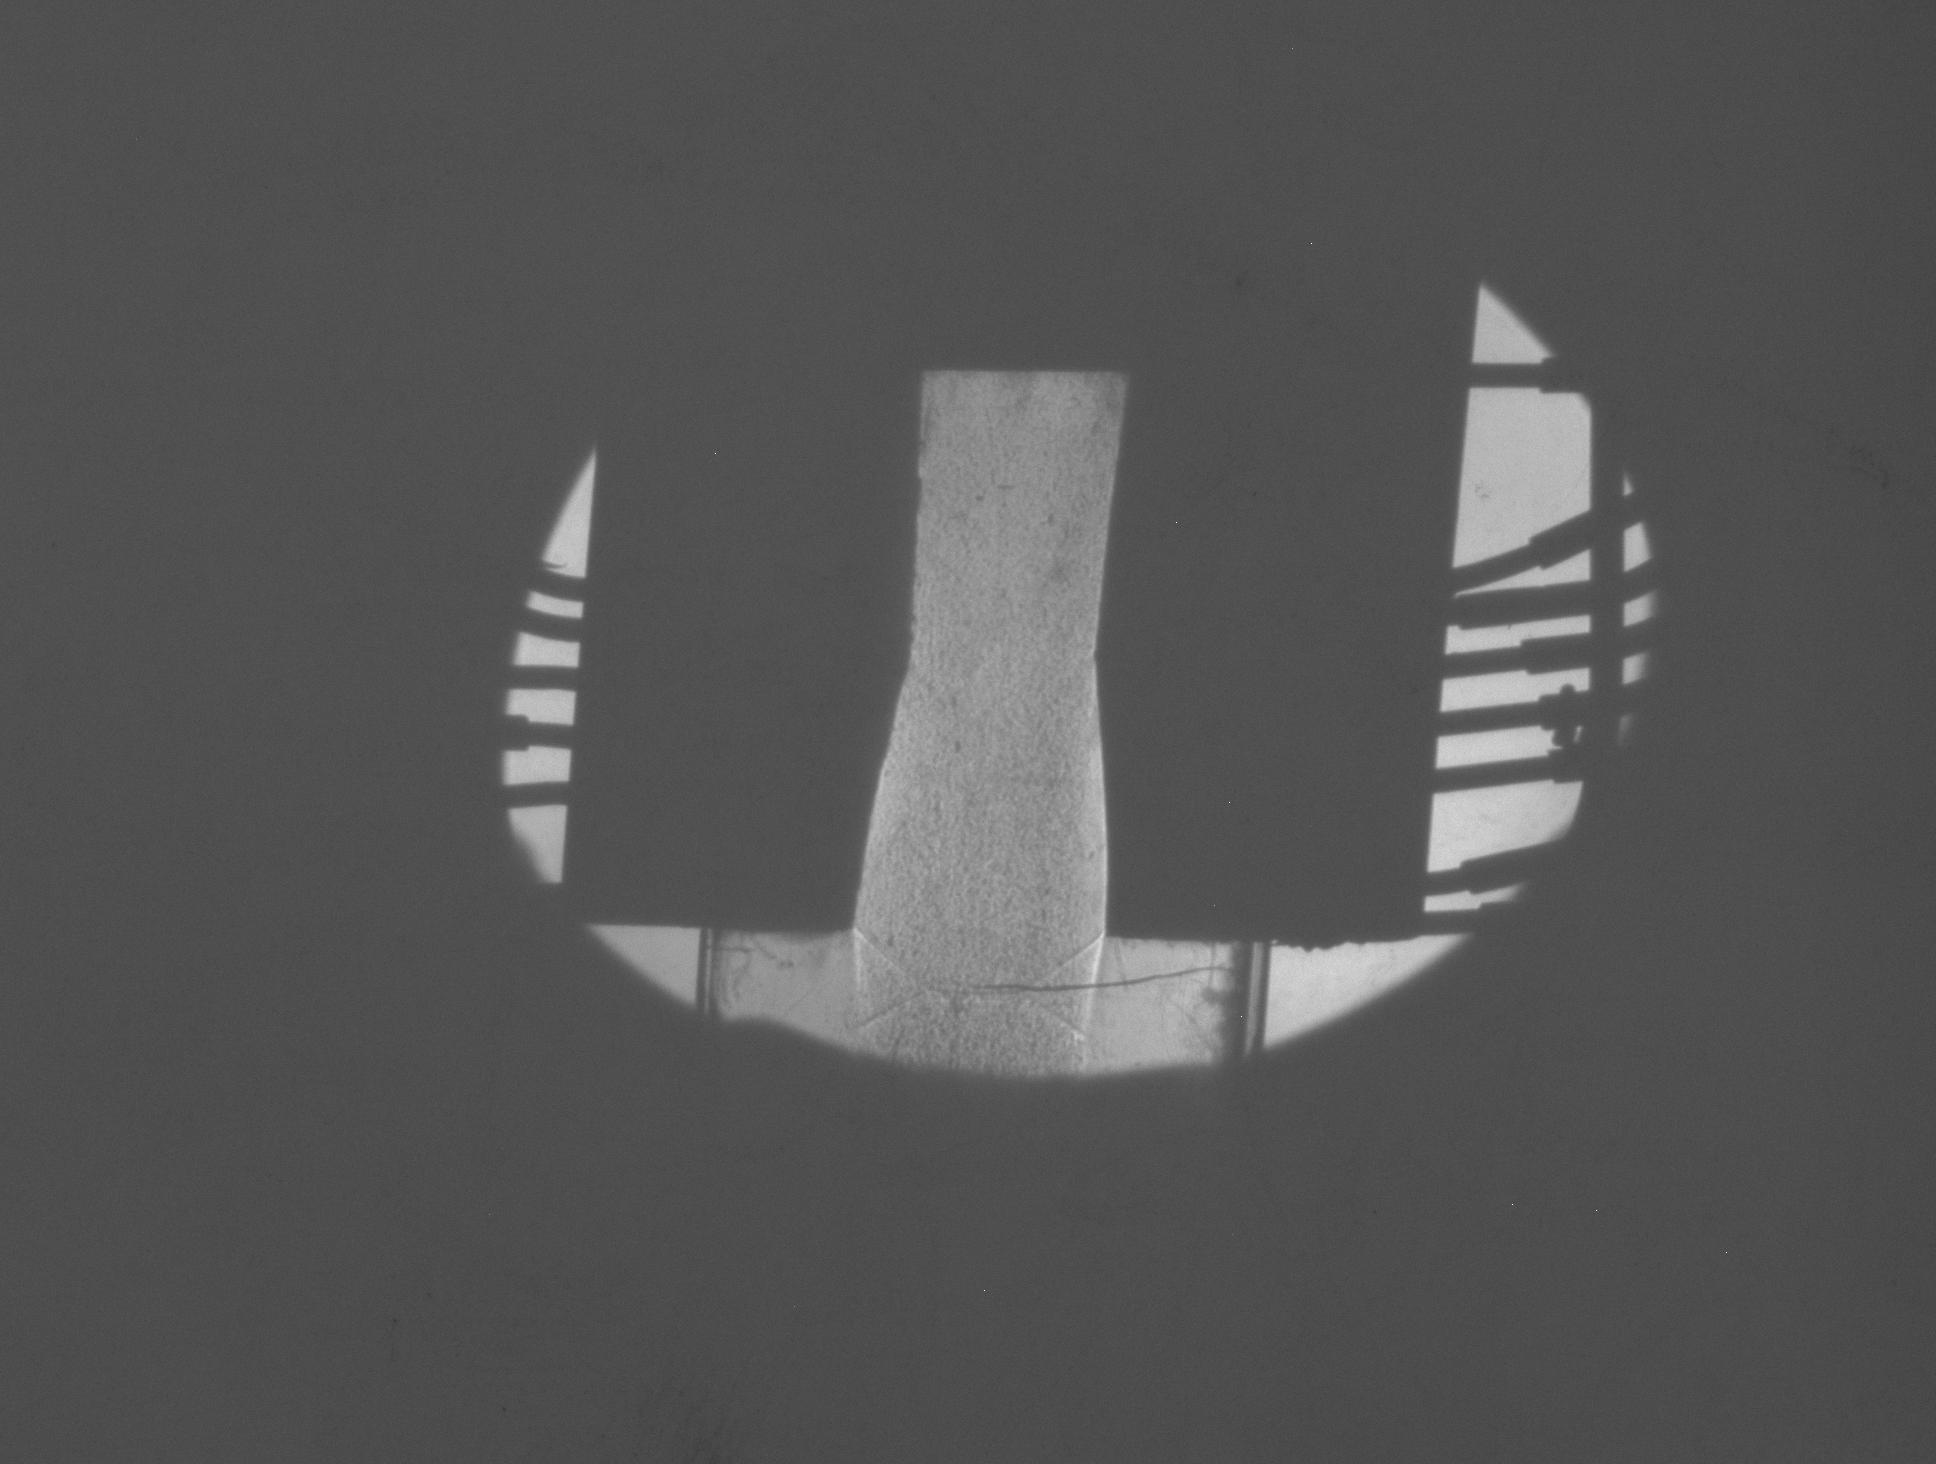
\includegraphics[width=\textwidth]{Figures/3-over-expanded_flow.tiff}
        \caption{Flow is over-expanded.}
        \label{fig:schlieren_over-expanded}
    \end{subfigure} \\
    \begin{subfigure}{0.49\textwidth}
        \centering
        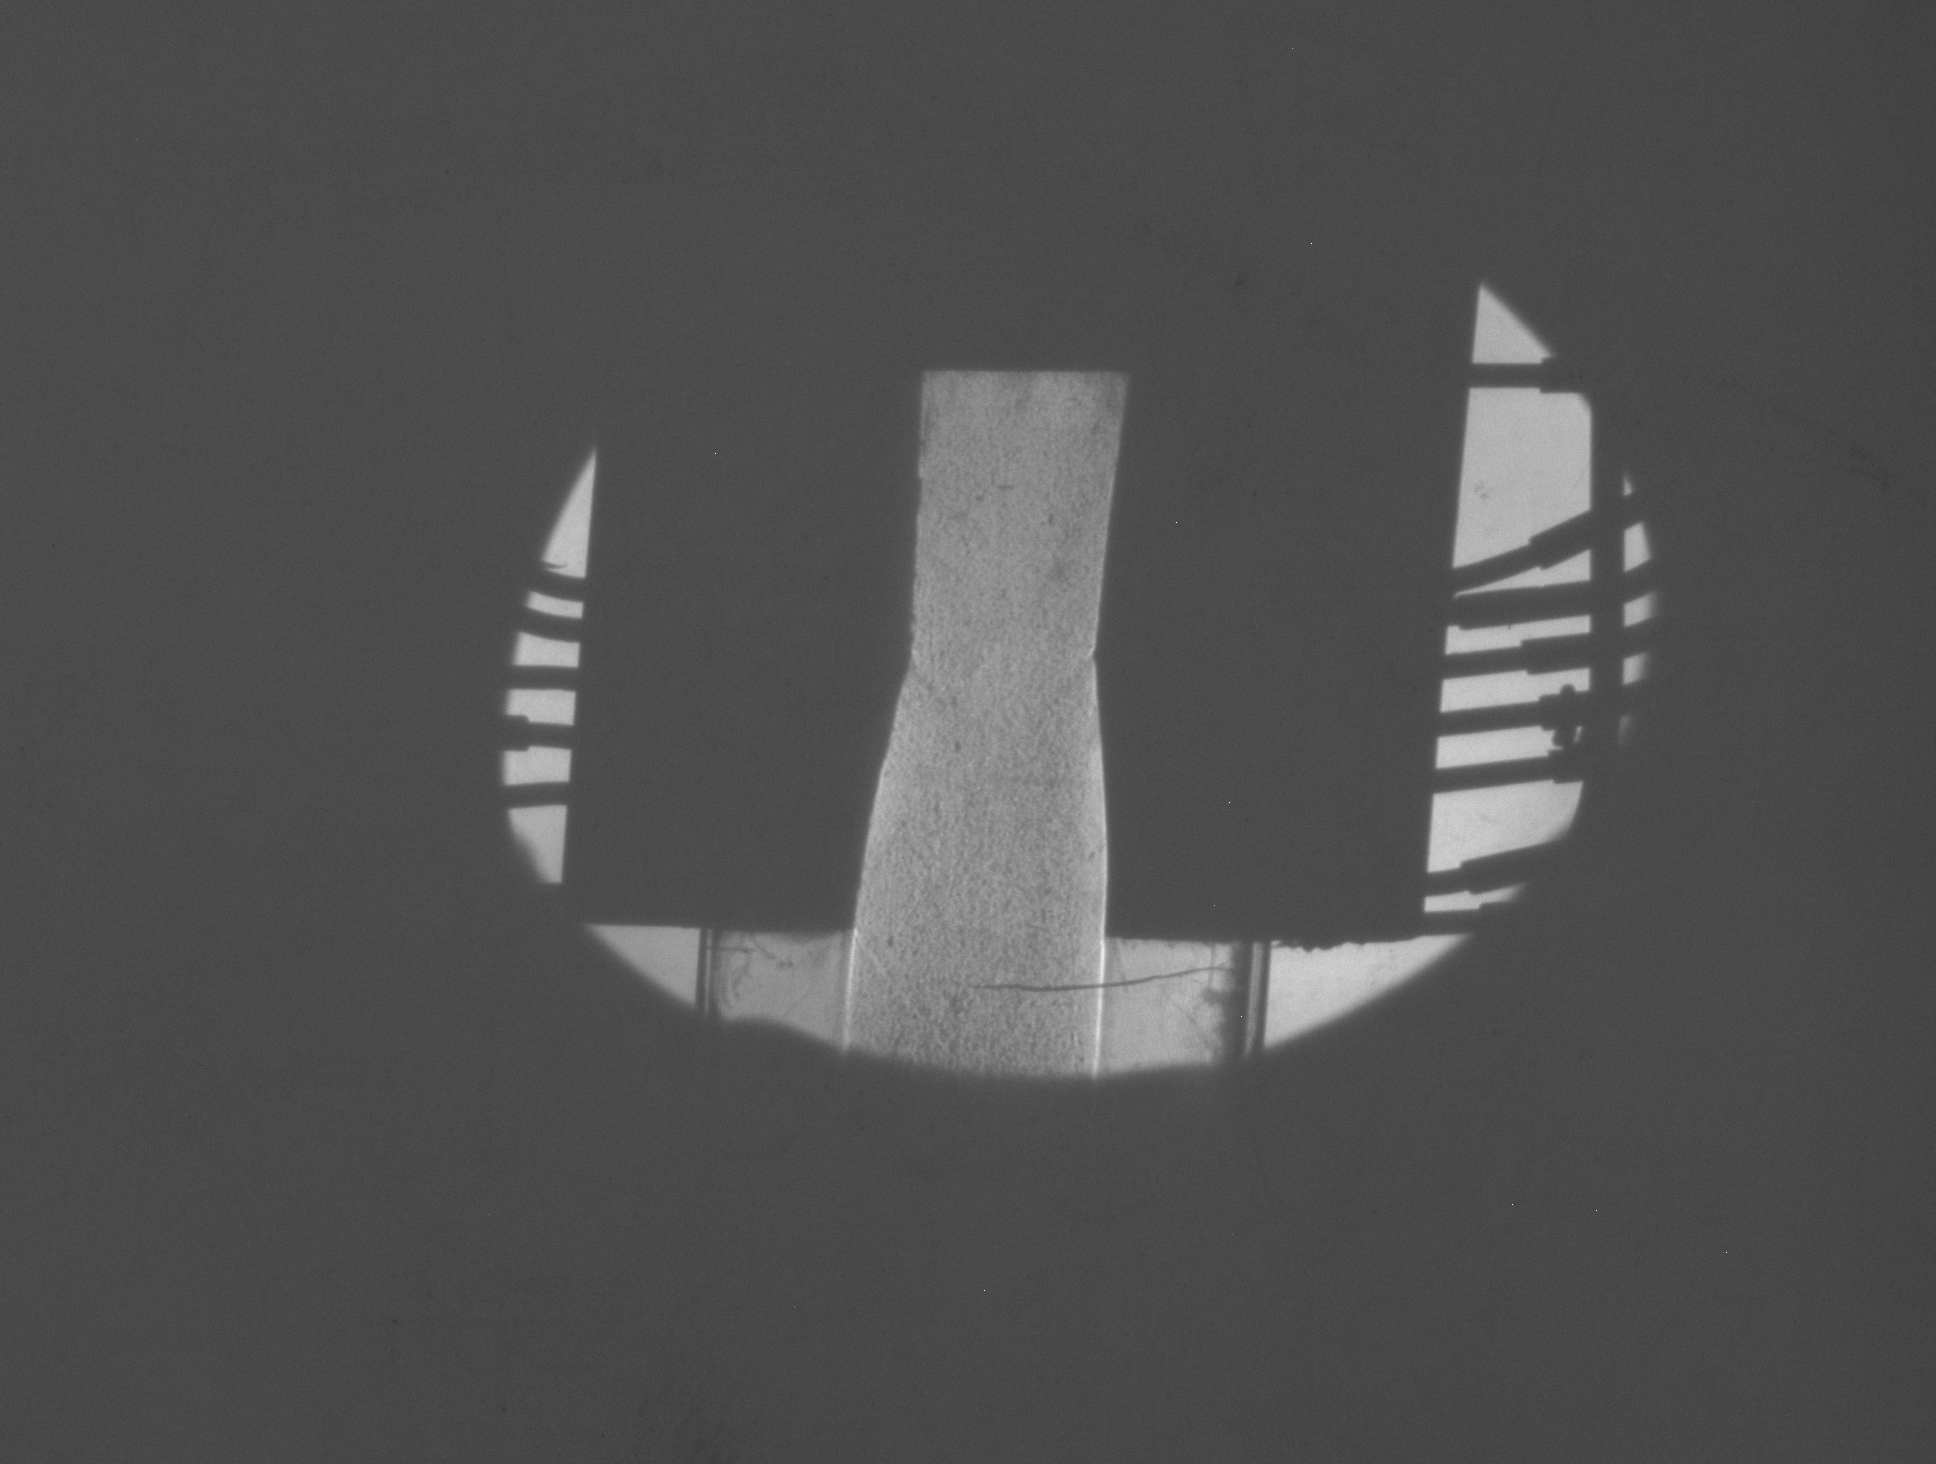
\includegraphics[width=\textwidth]{Figures/2-3rd_critical_condition.tiff}
        \caption{Flow is at the third critical position.}
        \label{fig:schlieren_third_critical}
    \end{subfigure}
    \begin{subfigure}{0.49\textwidth}
        \centering
        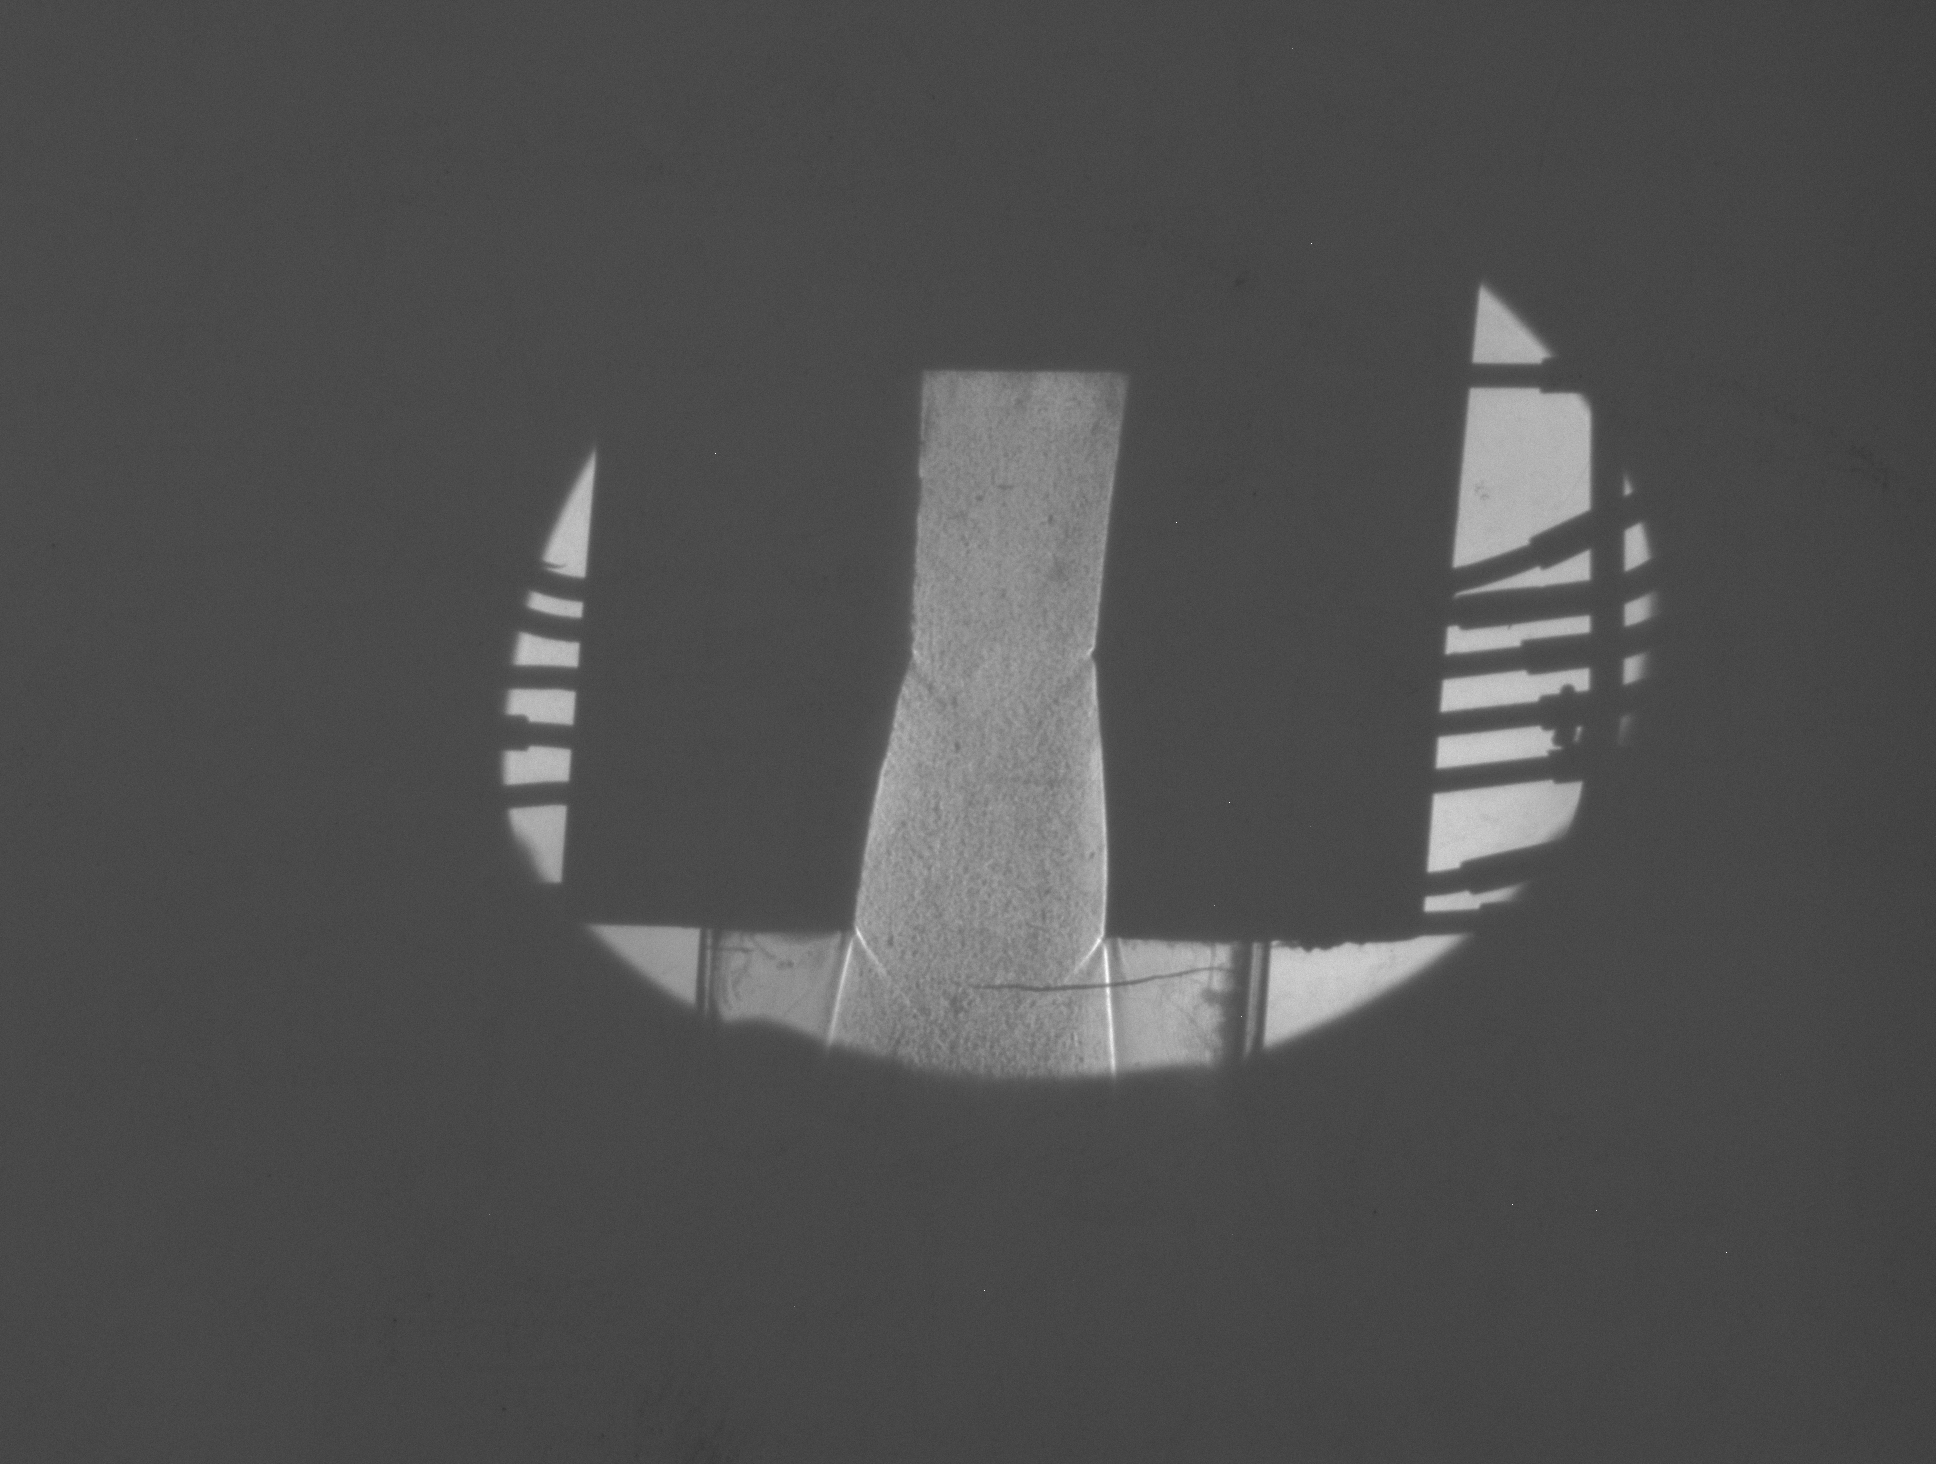
\includegraphics[width=\textwidth]{Figures/1-under-expanded_flow.tiff}
        \caption{Flow is under-expanded.}
        \label{fig:schlieren_under-expanded}
    \end{subfigure}
    \caption{Images captured by the camera in the Schlieren projection setup.}
    \label{fig:schlieren_image_captures}
\end{figure}